% =====================================================================
%  CHAPTER 4 (PART 1): MODEL EVALUATION RESULTS
%  The discussion that continues this chapter is in discussion.tex
% =====================================================================
\providecommand{\mpnet}{\texttt{paraphrase-\allowbreak multilingual-\allowbreak mpnet-\allowbreak base-\allowbreak v2}}
\providecommand{\cemodel}{\texttt{ms-marco-\allowbreak MiniLM-\allowbreak L-6-\allowbreak v2}}
\emergencystretch=3em
\providecommand{\pending}[1]{\textbf{[PENDING: #1]}}

\chapter{Results and Discussion}
\label{chap:results}

This chapter reports the results of the experiments described in Chapter~\ref{chap:methodology} and discusses what they mean. The results are presented first, in four parts. Section~\ref{sec:resenglish} evaluates restaurant ranking on the English RIRD benchmark, covering the fair comparison of BM25 and dense retrieval, the review-volume control, and the effect of changing the retrieval unit from review to sentence. Section~\ref{sec:resexplain} reports the two explanation experiments. Section~\ref{sec:resb3} reports the evaluation of the query-rewriting and cross-encoder extension, and Section~\ref{sec:resthai} reports the Thai sentence-level case study. The discussion of these results, including the comparison with other approaches in terms of performance, interpretability, and complexity, follows in Section~\ref{sec:discussion}.

% ---------------------------------------------------------------------
\section{English Ranking Results on RIRD}
\label{sec:resenglish}

All results in this section are computed on the 100 PMD queries and the 50 RIRD restaurants, using the aggregated binary relevance labels. Metric values are means over the 100 queries.

\subsection{Review-Level Comparison of BM25 and Dense Retrieval}
\label{sec:resreview}

Table~\ref{tab:reviewfull} reports every model evaluated at review level, sorted by nDCG@10. It includes the two proposal-phase baselines (BM25 on concatenated documents and the dense pooled vector), BM25 and dense retrieval with each of the five aggregation functions applied to review scores, and the three query-independent floors.

\begin{table}[htbp]
\centering
\caption{Review-Level Ranking Results on RIRD (100 Queries, 50 Restaurants)}
\label{tab:reviewfull}
\resizebox{\textwidth}{!}{%
\begin{tabular}{|l|c|c|c|c|c|c|c|c|}
\hline
\textbf{Model} & \textbf{MAP} & \textbf{MRR} & \textbf{nDCG@5} & \textbf{nDCG@10} & \textbf{R@5} & \textbf{R@10} & \textbf{P@5} & \textbf{P@10} \\
\hline
Dense, top-10 mean & 0.6083 & 0.7603 & 0.6493 & 0.6682 & 0.3503 & 0.5199 & 0.552 & 0.473 \\
Dense, top-5 mean & 0.6057 & 0.7465 & 0.6448 & 0.6676 & 0.3476 & 0.5178 & 0.554 & 0.472 \\
Dense, top-3 mean & 0.6013 & 0.7443 & 0.6380 & 0.6649 & 0.3454 & 0.5172 & 0.548 & 0.470 \\
Dense, pooled vector (v1) & 0.5853 & 0.7592 & 0.6337 & 0.6450 & 0.3406 & 0.4797 & 0.530 & 0.449 \\
Dense, mean & 0.5842 & 0.7502 & 0.6285 & 0.6423 & 0.3362 & 0.4730 & 0.524 & 0.448 \\
BM25, top-10 mean & 0.5765 & 0.7615 & 0.6218 & 0.6338 & 0.3358 & 0.4764 & 0.510 & 0.427 \\
Dense, max & 0.5643 & 0.7149 & 0.6006 & 0.6252 & 0.3157 & 0.4797 & 0.492 & 0.438 \\
BM25, concatenated doc (v1) & 0.5612 & 0.7690 & 0.6008 & 0.6211 & 0.3156 & 0.4501 & 0.462 & 0.407 \\
BM25, top-5 mean & 0.5659 & 0.7597 & 0.6077 & 0.6209 & 0.3242 & 0.4728 & 0.500 & 0.422 \\
BM25, top-3 mean & 0.5554 & 0.7494 & 0.5910 & 0.6114 & 0.3239 & 0.4606 & 0.484 & 0.420 \\
BM25, max & 0.5188 & 0.6910 & 0.5427 & 0.5753 & 0.2964 & 0.4327 & 0.458 & 0.404 \\
BM25, mean & 0.5067 & 0.6358 & 0.5190 & 0.5487 & 0.2851 & 0.4229 & 0.422 & 0.377 \\
\hline
Popularity (leave-one-out) & 0.4257 & 0.4359 & 0.4491 & 0.4840 & 0.2085 & 0.3406 & 0.430 & 0.410 \\
Review count & 0.3490 & 0.5045 & 0.3607 & 0.3735 & 0.1211 & 0.2015 & 0.296 & 0.281 \\
Random (expected) & 0.3221 & 0.4284 & 0.3192 & 0.3478 & 0.1017 & 0.2033 & 0.269 & 0.270 \\
\hline
\end{tabular}}

\vspace{2pt}
\footnotesize\textit{Note.} R = recall, P = precision. Rows above the rule are retrieval models; rows below the rule are query-independent floors.
\end{table}

Three patterns are visible in Table~\ref{tab:reviewfull}. First, dense retrieval with the top-10 mean aggregation achieves the highest nDCG@10 (0.668) and the highest MAP (0.608) of all review-level models. Second, dense retrieval outperforms BM25 under every one of the five aggregation functions, and these differences remain significant after Holm correction. For example, with the top-10 mean, dense retrieval reaches an nDCG@10 of 0.668 compared with 0.634 for BM25, and with the plain mean it reaches 0.642 compared with 0.549. Third, the choice of aggregation matters for both retrieval models: the top-$k$ means are consistently better than the maximum and the mean over all reviews. For BM25, the mean over all reviews is the weakest aggregation (nDCG@10 of 0.549), and for dense retrieval the maximum is weaker than every top-$k$ mean (0.625 versus 0.665 to 0.668).

All retrieval models clearly outperform the query-independent floors. The random ranking reaches an nDCG@10 of 0.348, ranking by review count reaches 0.374, and the leave-one-out popularity ranking reaches 0.484. The popularity floor is notable because it ranks restaurants without ever reading the query, and it already attains a precision at ten of 0.410. This shows that part of the relevance in PMD is explained by some restaurants simply being relevant to many different queries, and it makes clear why a model must be judged against these floors and not only against another retrieval model.

\subsection{Proposed Model Versus Baseline}
\label{sec:resheadline}

Table~\ref{tab:headline} brings together the baseline, the proposal-phase dense baseline, and the proposed model at review and sentence level, with 95\% bootstrap confidence intervals where they are available.

\begin{table}[htbp]
\centering
\caption{Baseline and Proposed Models on RIRD}
\label{tab:headline}
\small
\begin{tabular}{|p{0.31\textwidth}|p{0.15\textwidth}|p{0.21\textwidth}|p{0.21\textwidth}|}
\hline
\textbf{Model} & \textbf{Unit} & \textbf{nDCG@10 [95\% CI]} & \textbf{MAP [95\% CI]} \\
\hline
BM25, concatenated doc (baseline) & Restaurant & 0.621 [0.578, 0.663] & 0.561 [0.510, 0.612] \\
\hline
Dense, pooled vector (v1) & Restaurant & 0.645 [0.603, 0.687] & 0.585 [0.531, 0.639] \\
\hline
BM25, top-10 mean & Review & 0.634 [0.590, 0.677] & 0.577 [0.525, 0.626] \\
\hline
Dense, top-10 mean & Review & 0.668 [0.625, 0.711] & 0.608 [0.555, 0.662] \\
\hline
BM25, top-10 mean & Sentence & 0.609 [0.567, 0.652] & 0.536 [0.484, 0.588] \\
\hline
\textbf{Dense, top-10 mean (proposed)} & \textbf{Sentence} & \textbf{0.682 [0.638, 0.723]} & \textbf{0.618 [0.564, 0.671]} \\
\hline
\end{tabular}

\vspace{2pt}
\footnotesize\textit{Note.} Confidence intervals are percentile bootstrap intervals over the 100 queries (95\%, 10,000 resamples, seed 42).
\end{table}

The proposed sentence-level dense model with top-10 mean aggregation reaches an nDCG@10 of 0.682 and a MAP of 0.618. Relative to the BM25 baseline on concatenated documents (nDCG@10 of 0.621 and MAP of 0.561), this is an absolute improvement of 0.060 in nDCG@10 and 0.057 in MAP. The confidence intervals of the baseline and of the proposed model overlap, so the improvement should be read as a consistent gain over the baseline and not as a decisive one on this sample of 100 queries. Within the comparisons that hold the retrieval unit and aggregation fixed, the advantage of dense retrieval over BM25 is statistically reliable, as reported in Section~\ref{sec:resreview}.

\subsection{Effect of Review Volume}
\label{sec:resvolume}

The volume control of Section~\ref{sec:volumecontrol} subsampled every restaurant to 400 reviews. After this control the Pearson correlation between a restaurant's score and its review count fell to near zero, between $-0.009$ and $+0.019$ across the variants, and the change in nDCG@10 was at most 0.011. This indicates that the aggregation functions are not materially biased towards restaurants with many reviews in this dataset, and that the ranking differences reported in Table~\ref{tab:reviewfull} cannot be attributed to review volume. The review-count floor in Table~\ref{tab:reviewfull} nevertheless scores slightly above the random floor (0.374 versus 0.348), so review volume is weakly related to relevance on its own.

\subsection{Review Level Versus Sentence Level}
\label{sec:resa5}

Table~\ref{tab:a5} reports the paired comparison of review-level and sentence-level nDCG@10 for the variants for which the result is available, and Figure~\ref{fig:a5forest} shows the paired differences for all shared variants.

\begin{table}[htbp]
\centering
\caption{Review-Level Versus Sentence-Level nDCG@10 (Paired Randomisation Test)}
\label{tab:a5}
\small
\begin{tabular}{|p{0.27\textwidth}|c|c|c|c|}
\hline
\textbf{Variant} & \textbf{Review} & \textbf{Sentence} & \textbf{$\Delta$ (sent.\ $-$ rev.)} & \textbf{Holm $p$} \\
\hline
Dense, top-10 mean & 0.668 & 0.682 & $+0.013$ & 1.00 \\
\hline
BM25, top-10 mean & 0.634 & 0.609 & $-0.025$ & 0.581 \\
\hline
Dense, mean & 0.642 & 0.587 & $-0.055$ & $<0.001$ \\
\hline
\end{tabular}

\vspace{2pt}
\footnotesize\textit{Note.} $\Delta$ is the mean per-query difference. The test is a two-sided paired randomisation test with 10,000 permutations and Holm correction across all shared variants. Only the variants discussed in the text are shown.
\end{table}

\begin{figure}[htbp]
    \centering
    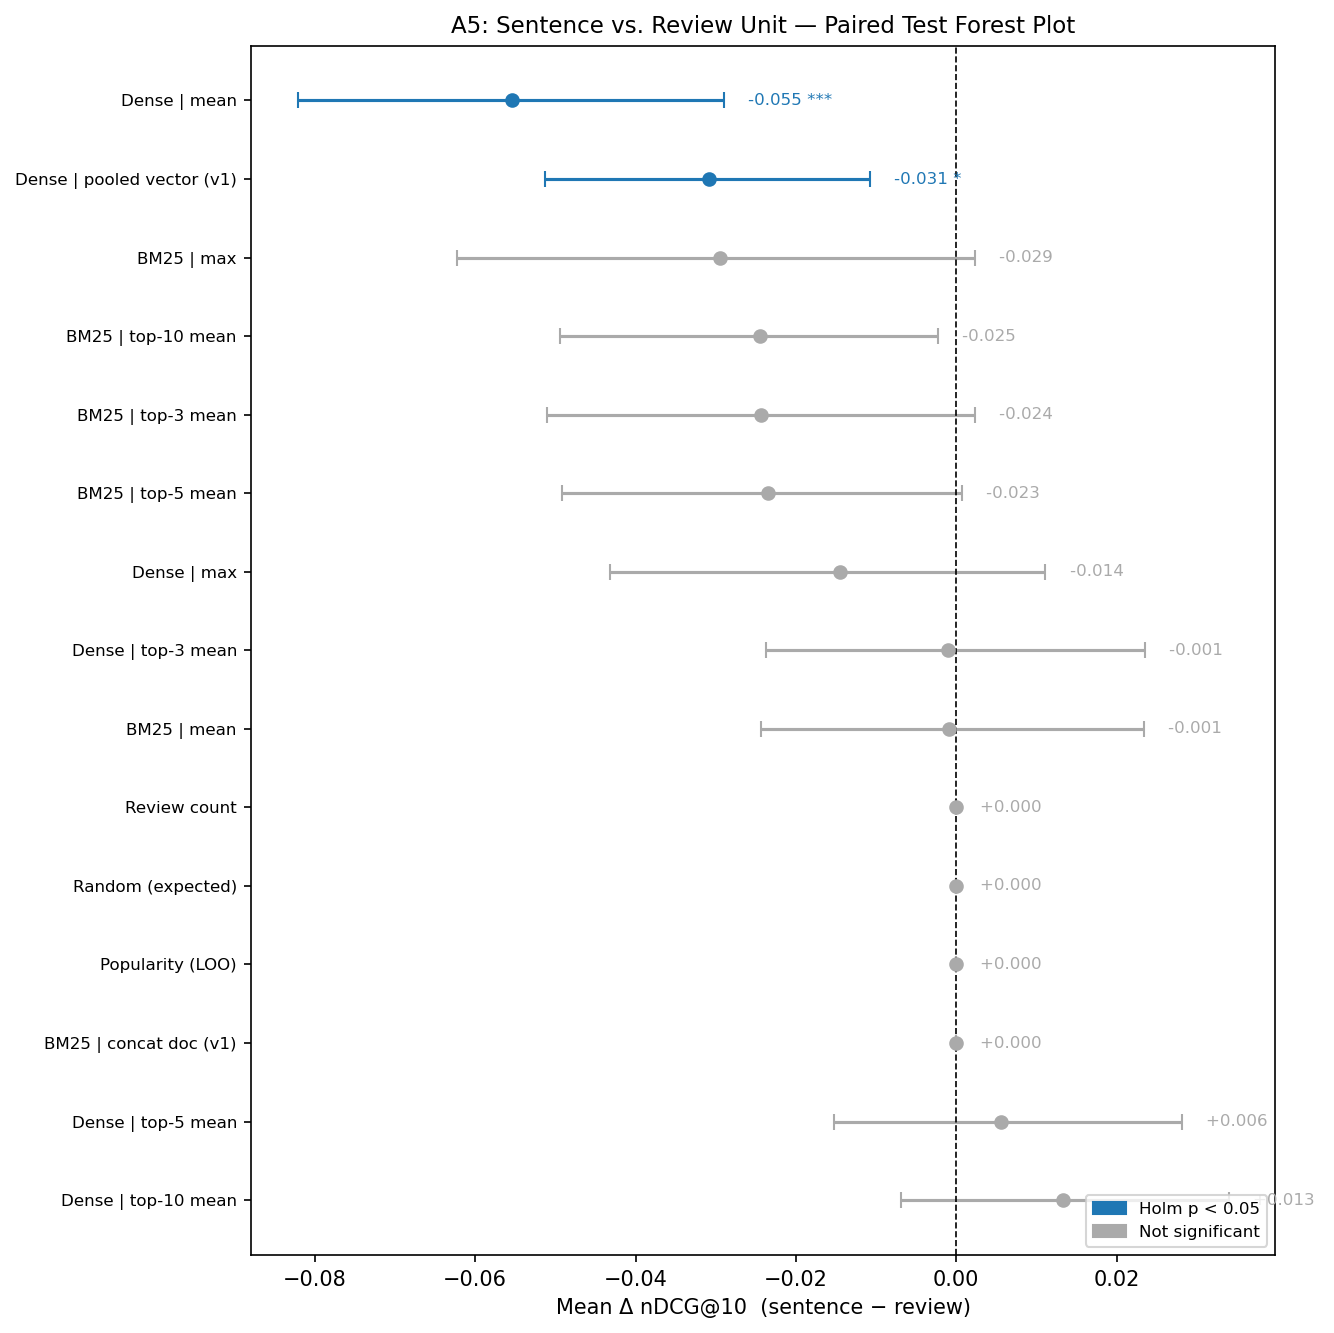
\includegraphics[width=0.85\textwidth]{figures/a5_forest_plot.png}
    \caption{Paired difference in nDCG@10 between sentence level and review level for each shared variant.}
    \label{fig:a5forest}
\end{figure}

Switching the retrieval unit from review to sentence does not produce a significant improvement for any variant after Holm correction. The dense top-10 mean variant shows the largest positive gap ($\Delta=+0.013$) but it is not significant (Holm $p=1.00$), whereas the dense mean aggregation becomes significantly worse at sentence level ($\Delta=-0.055$, Holm $p<0.001$). At sentence level, dense retrieval still outperforms BM25 for the maximum and for every top-$k$ mean (Holm $p\le0.004$), while the difference under the plain mean is not significant ($p=0.072$). In short, the sentence-level proposed model has the highest nDCG@10 of all models, but this is mainly because sentence-level scores can be aggregated by the top-$k$ mean, and not because sentence units are significantly better in themselves. The benefit of the sentence unit for this project is therefore primarily explainability, since sentences are the natural units to show a user as evidence, and not ranking accuracy.

% ---------------------------------------------------------------------
\section{Explanation Evaluation Results}
\label{sec:resexplain}

\subsection{Automatic Faithfulness Test}
\label{sec:resb1}

Table~\ref{tab:b1} and Figure~\ref{fig:b1} report the faithfulness test on 300 query--restaurant pairs. The mean rank drop was identical for the shown sentences and for random sentences (48.0 in both cases), so the mean faithfulness gap was exactly 0.000, with a bootstrap confidence interval of [0.000, 0.000] and a one-tailed $p$-value of 1.0. Deleting either set of sentences reduced nDCG@10 from 0.682 to 0.379, a loss of 0.302.

\begin{table}[htbp]
\centering
\caption{Automatic Faithfulness Test Summary}
\label{tab:b1}
\small
\begin{tabular}{|p{0.52\textwidth}|p{0.25\textwidth}|}
\hline
\textbf{Quantity} & \textbf{Value} \\
\hline
Query--restaurant pairs tested & 300 \\
\hline
Mean rank drop, shown sentences deleted & 48.0 \\
\hline
Mean rank drop, random sentences deleted & 48.0 \\
\hline
Mean faithfulness gap [95\% CI] & 0.000 [0.000, 0.000] \\
\hline
One-tailed $p$-value & 1.0 \\
\hline
nDCG@10, baseline & 0.682 \\
\hline
nDCG@10, after shown deletion & 0.379 \\
\hline
nDCG@10, after random deletion & 0.379 \\
\hline
\end{tabular}
\end{table}

\begin{figure}[htbp]
    \centering
    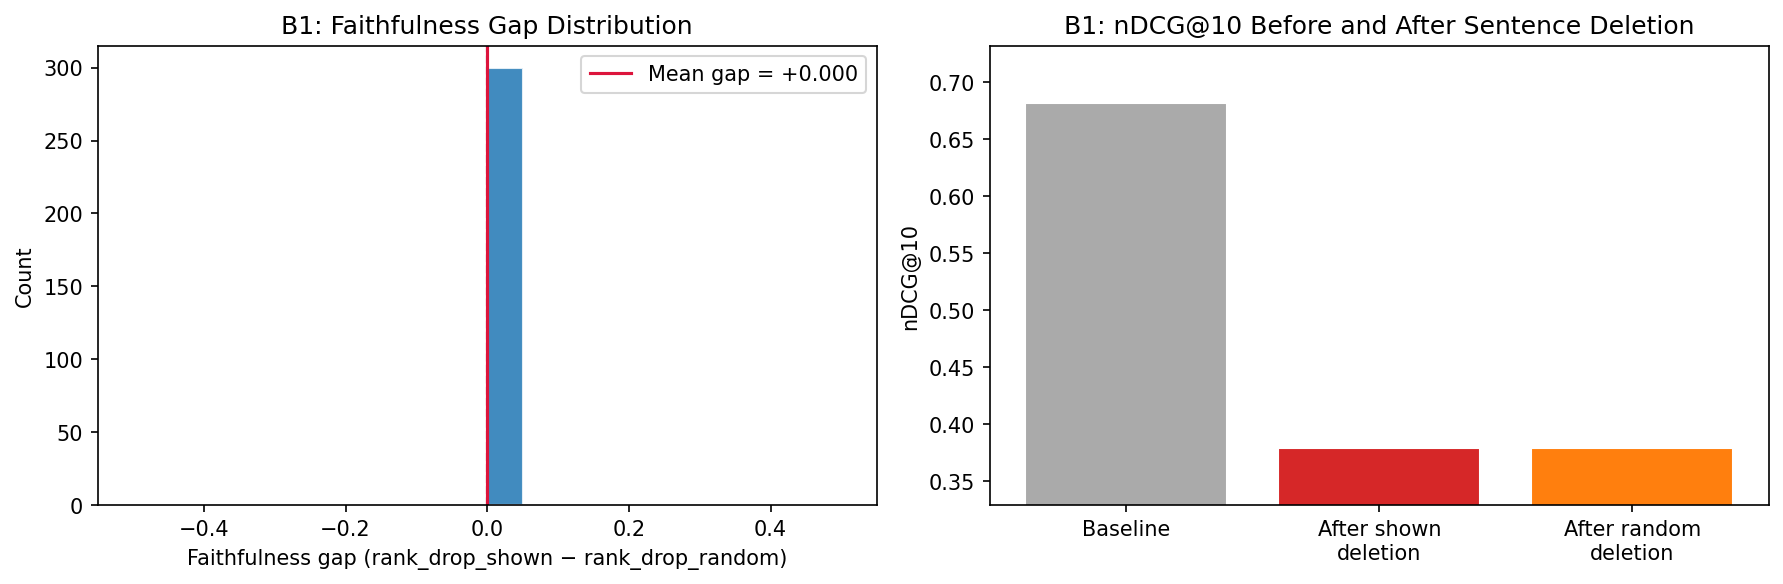
\includegraphics[width=\textwidth]{figures/b1_faithfulness_plot.png}
    \caption{Faithfulness gap distribution (left) and nDCG@10 before and after sentence deletion (right).}
    \label{fig:b1}
\end{figure}

The test is therefore \emph{inconclusive} and not a demonstration of faithfulness or of its absence. Our interpretation is that the evidence store used in this experiment is small (the top ten sentences of each restaurant), so that deleting the shown sentences and deleting the same number of random sentences from the store hit the same sentences, which makes the two conditions indistinguishable by construction. A redesigned test with a much larger candidate pool per restaurant would be needed to measure whether the displayed sentences carry more weight than other sentences.

\subsection{Human Support Rating}
\label{sec:resb2}

The human support sheet contains 375 items (25 queries $\times$ 3 restaurants $\times$ 5 sentences). Both annotators completed their labelling in full. Annotator~1 (Sam) labelled all 375 items; annotator~2 (Ton) labelled a 40-item subset for inter-annotator agreement. Of the 375 items labelled by annotator~1, 148 were rated~0 (not supporting), 143 were rated~1 (partially supporting), and 84 were rated~2 (clearly supporting), so 227 of 375 items (60.5\%) were rated as at least partially supporting the restaurant for the query (label~$\ge 1$), and 84 of 375 (22.4\%) were rated as clearly supporting (label~$=2$). On the 40-pair overlap between the two annotators, exact agreement was 70.0\% and Cohen's $\kappa$ was 0.544, interpreted as moderate agreement.

The per-query support rates (annotator~1) vary widely. Some queries achieved 100\% support (for example ``A date place for valentines with affordable drinks'' and ``I want a place to hang out with my work friends''), while others received 0\% support (for example ``I am looking for a restaurant with no waiting line'', ``Late for work and I need to fill up before leaving'', and ``outdoor space without live music''). The two zero-support queries related to waiting reflect the negation blindness of the bi-encoder: the retrieved sentences discuss busy restaurants or long waits, which is the opposite of what the query requests. The B3 fix addresses this for the live system but the pre-computed evidence for these queries was produced before the fix.

\begin{table}[htbp]
\centering
\caption{Human Support Ratings of Displayed Sentences (Full Sheet)}
\label{tab:b2}
\small
\begin{tabular}{|p{0.42\textwidth}|p{0.40\textwidth}|}
\hline
\textbf{Quantity} & \textbf{Value} \\
\hline
Items in the rating sheet & 375 \\
\hline
Items labelled by annotator 1 (Sam) & 375 / 375 (complete) \\
\hline
Items labelled by annotator 2 (Ton) & 40 / 375 (agreement subset) \\
\hline
Rated 0 / 1 / 2 (annotator 1, full sheet) & 148 / 143 / 84 \\
\hline
Share rated as supporting ($\ge 1$) & 60.5\% (227\,/\,375) \\
\hline
Share rated as clearly supporting ($=2$) & 22.4\% (84\,/\,375) \\
\hline
Exact agreement on 40-pair overlap & 70.0\% \\
\hline
Cohen's $\kappa$ on 40-pair overlap & 0.544 (moderate) \\
\hline
\end{tabular}
\end{table}

% ---------------------------------------------------------------------
\section{Query Rewriting and Cross-Encoder Re-ranking}
\label{sec:resb3}

The combined extension of Section~\ref{sec:b3} was evaluated on all 100 queries against the sentence-level dense baseline with the top-10 mean aggregation. All 100 queries were rewritten, and the cross-encoder was applied to all of them in this experiment. Table~\ref{tab:b3} and Figure~\ref{fig:b3} compare the two configurations.

\begin{table}[htbp]
\centering
\caption{Baseline Versus Rewriting and Cross-Encoder Re-ranking (All 100 Queries)}
\label{tab:b3}
\small
\begin{tabular}{|l|c|c|c|}
\hline
\textbf{Metric} & \textbf{Baseline} & \textbf{Improved} & \textbf{Change} \\
\hline
nDCG@10 & 0.6815 & 0.6575 & $-0.0240$ \\
\hline
nDCG@5 & 0.6609 & 0.6563 & $-0.0046$ \\
\hline
MAP & 0.6177 & 0.5859 & $-0.0318$ \\
\hline
MRR & 0.7730 & 0.7733 & $+0.0003$ \\
\hline
P@5 & 0.560 & 0.542 & $-0.018$ \\
\hline
P@10 & 0.487 & 0.457 & $-0.030$ \\
\hline
Recall@5 & 0.3463 & 0.3403 & $-0.0060$ \\
\hline
Recall@10 & 0.5205 & 0.4695 & $-0.0510$ \\
\hline
\end{tabular}
\end{table}

\begin{figure}[htbp]
    \centering
    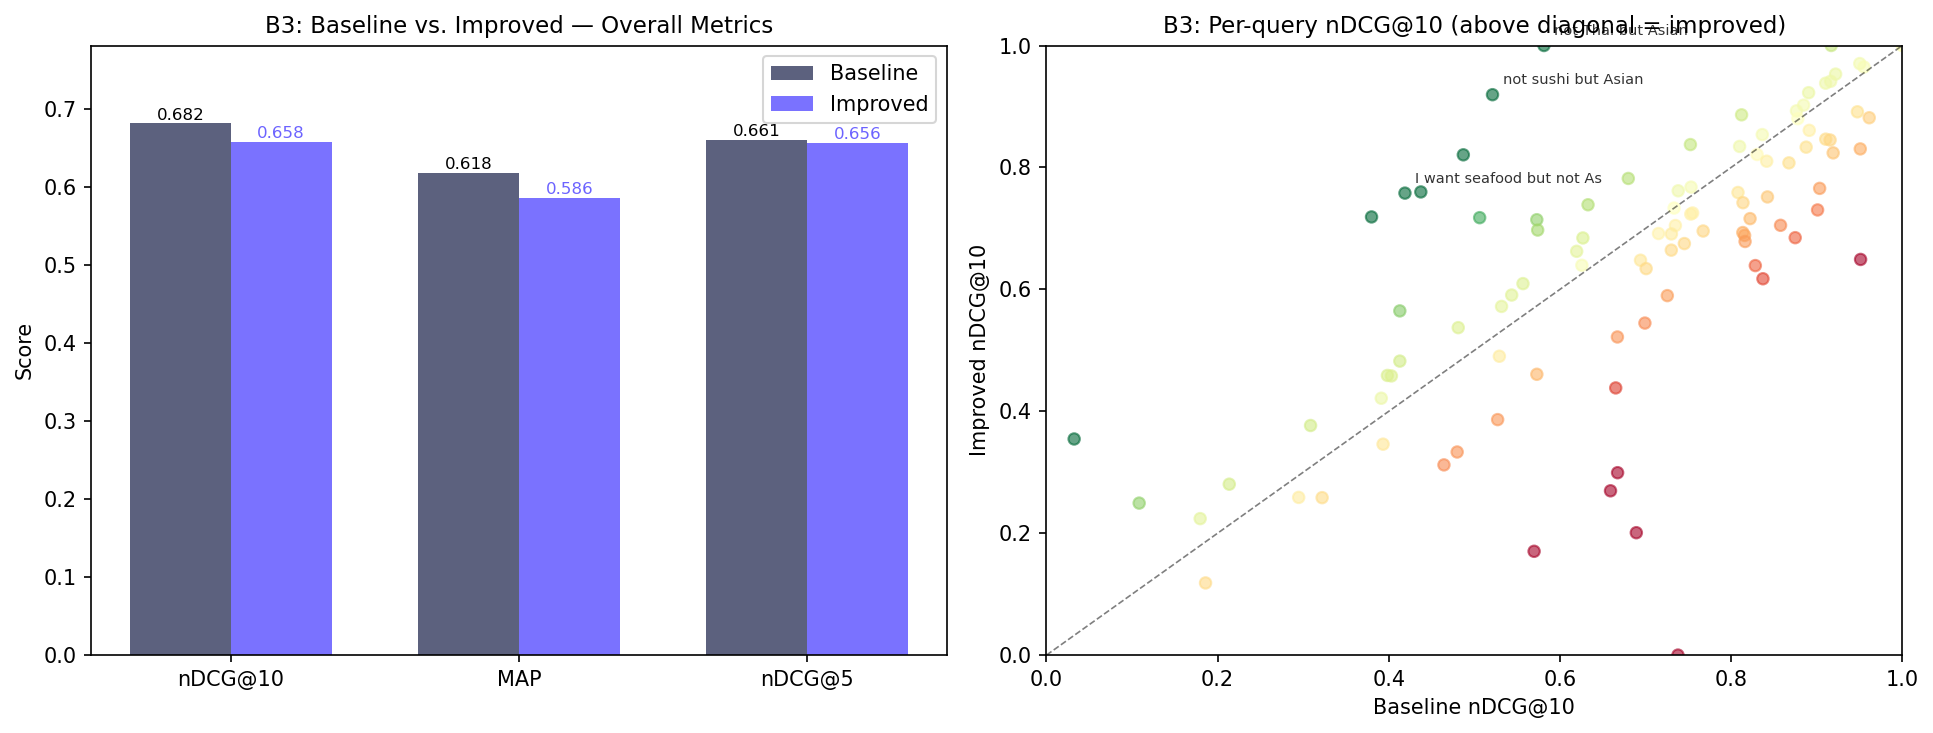
\includegraphics[width=\textwidth]{figures/b3_comparison_plot.png}
    \caption{Overall metrics for the baseline and the improved system (left) and per-query nDCG@10 (right).}
    \label{fig:b3}
\end{figure}

Applied to every query, the extension did not improve overall ranking quality: nDCG@10 fell from 0.682 to 0.658 and MAP from 0.618 to 0.586, while MRR was essentially unchanged. At the level of individual queries the picture is mixed. Of the 100 queries, 44 improved, 53 degraded, and 3 were unchanged in nDCG@10, with a mean change of $-0.024$ and a median change of $-0.030$. The scatter plot in Figure~\ref{fig:b3} shows that a group of queries gained substantially (points far above the diagonal), while another group lost substantially.

Table~\ref{tab:b3queries} lists the five largest gains and the five largest losses. The largest gains are concentrated in queries that contain an explicit exclusion, such as ``not Thai but Asian'', ``not sushi but Asian'', and ``I want seafood but not Asian'', for which the rewrite spells out the wanted alternatives (for example ``Chinese Japanese Korean Vietnamese Indian''). The two remaining gains, ``I am on a budget'' and ``I prefer a place that offers cash discounts'', are not negations, which shows that rewriting can also help vague or idiomatic queries. The largest losses are plain positive queries, such as ``An ice cream shop with bubble tea'', whose nDCG@10 fell from 0.738 to 0.000, together with two queries that contain a negation or contrast (``I am vegan but my friends want good steaks'' and ``I have a car but I don't want to pay for parking'').

\begin{table}[htbp]
\centering
\caption{Queries With the Largest Change in nDCG@10 Under Rewriting and Cross-Encoder Re-ranking}
\label{tab:b3queries}
\footnotesize
\begin{tabular}{|p{0.43\textwidth}|c|c|c|}
\hline
\textbf{Query} & \textbf{Baseline} & \textbf{Improved} & \textbf{Change} \\
\hline
\multicolumn{4}{|l|}{\textit{Largest gains}} \\
\hline
not Thai but Asian & 0.581 & 1.000 & $+0.419$ \\
\hline
not sushi but Asian & 0.521 & 0.919 & $+0.398$ \\
\hline
I prefer a place that offers cash discounts & 0.380 & 0.719 & $+0.339$ \\
\hline
I want seafood but not Asian & 0.419 & 0.758 & $+0.339$ \\
\hline
I am on a budget & 0.487 & 0.821 & $+0.334$ \\
\hline
\multicolumn{4}{|l|}{\textit{Largest losses}} \\
\hline
An ice cream shop with bubble tea & 0.738 & 0.000 & $-0.738$ \\
\hline
I am vegan but my friends want good steaks & 0.689 & 0.201 & $-0.488$ \\
\hline
I have a car but I don't want to pay for parking & 0.570 & 0.170 & $-0.400$ \\
\hline
A fancy, but affordable place & 0.659 & 0.270 & $-0.390$ \\
\hline
I am looking for a bar on the lakeshore & 0.667 & 0.299 & $-0.368$ \\
\hline
\end{tabular}
\end{table}

Two limitations of this experiment must be kept in mind. First, query rewriting and cross-encoder re-ranking were evaluated together, so the results cannot show which of the two components is responsible for the gains and for the losses. Second, the selective strategy used in the live system, which activates the cross-encoder only for queries with explicit negation or exclusion patterns, has not been evaluated as a separate configuration. The results above are for the cross-encoder applied to all queries.

% ---------------------------------------------------------------------
\section{Thai Sentence-Level Results}
\label{sec:resthai}

\subsection{Pool and Label Distribution}
\label{sec:resthaipool}

For each of the 24 frozen Thai queries, the top ten sentences of BM25 and of dense retrieval were retrieved from the 93,810 sentences of the 10,000-review Wongnai sample and merged into a blind pool of 452 pairs (Table~\ref{tab:thaipool}). Of these, 184 pairs (40.7\%) were labelled 0, 180 pairs (39.8\%) were labelled 1, and 88 pairs (19.5\%) were labelled 2. The two systems retrieve largely different sentences, sharing only 1.2 sentences on average within their top ten lists. One query has no sentence with a positive label in its pool.

\begin{table}[htbp]
\centering
\caption{Thai Annotation Pool}
\label{tab:thaipool}
\small
\begin{tabular}{|p{0.50\textwidth}|p{0.30\textwidth}|}
\hline
\textbf{Quantity} & \textbf{Value} \\
\hline
Frozen Thai queries & 24 \\
\hline
Retrieval corpus (sentences) & 93,810 \\
\hline
Labelled query--sentence pairs & 452 \\
\hline
Pairs per query (mean, range) & 18.8 (13--20) \\
\hline
Label 0 / 1 / 2 & 184 / 180 / 88 \\
\hline
Mean shared sentences in the two top-10 lists & 1.2 \\
\hline
\end{tabular}
\end{table}

\subsection{Retrieval Quality}
\label{sec:resthaiquality}

Table~\ref{tab:thaimetrics} compares the two systems on the 24 queries. BM25 obtains a higher mean score than dense retrieval on every metric, with an nDCG@10 of 0.654 versus 0.549, a lenient precision at ten of 0.667 versus 0.558, and a strict precision at ten of 0.258 versus 0.163. However, none of these differences is statistically significant after Holm correction: for nDCG@10 the dense-minus-BM25 difference is $-0.105$ with a 95\% confidence interval of $[-0.298, +0.093]$ (Holm $p=0.57$), and the intervals of the other two metrics also contain zero.

\begin{table}[htbp]
\centering
\caption{BM25 Versus Dense Retrieval on Thai Sentences (24 Queries)}
\label{tab:thaimetrics}
\small
\begin{tabular}{|p{0.27\textwidth}|c|c|p{0.17\textwidth}|c|}
\hline
\textbf{Metric} & \textbf{BM25} & \textbf{Dense} & \textbf{Difference [95\% CI]} & \textbf{Holm $p$} \\
\hline
nDCG@10 & 0.654 & 0.549 & $-0.105$ [$-0.298$, $0.093$] & 0.57 \\
\hline
P@10 (label $\ge 1$) & 0.667 & 0.558 & $-0.108$ [$-0.292$, $0.075$] & 0.57 \\
\hline
P@10 (label $=2$) & 0.258 & 0.163 & $-0.096$ [$-0.212$, $0.029$] & 0.47 \\
\hline
\end{tabular}

\vspace{2pt}
\footnotesize\textit{Note.} Difference is dense minus BM25, with paired bootstrap confidence intervals over the 24 queries.
\end{table}

A breakdown by query type shows where the gap comes from. For queries that combine several taste requirements, BM25 achieves a strict precision at ten of 0.325 compared with 0.125 for dense retrieval, and the confidence interval of this difference excludes zero. For queries with a negated preference, the two systems are essentially tied in nDCG@10 (0.574 for BM25 versus 0.607 for dense retrieval).

\subsection{Annotation Agreement}
\label{sec:resthaiagree}

On the 60-pair subset that received a second round of labels, the agreement with the first round is high: Cohen's $\kappa$ is 0.837, the weighted $\kappa$ is 0.869, and 90\% of the labels match exactly. Because the second round was drafted by a language model and then reviewed by the same team member who produced the first round, this agreement measures the consistency of the labelling guidelines and not the agreement of two independent human annotators. It should be interpreted with that limitation in mind.

% ---------------------------------------------------------------------
\section{Summary of Results}
\label{sec:ressummary}

The main quantitative findings of the English and Thai experiments are summarised in Table~\ref{tab:ressummary}. They are interpreted in the discussion that follows.

\begin{table}[htbp]
\centering
\caption{Summary of Main Results by Research Question}
\label{tab:ressummary}
\small
\begin{tabular}{|p{0.20\textwidth}|p{0.72\textwidth}|}
\hline
\textbf{Question} & \textbf{Main result} \\
\hline
Fair fusion & Dense beats BM25 under every aggregation at review level; the top-10 mean is best (nDCG@10 0.668). The sentence-level proposed model reaches nDCG@10 0.682 and MAP 0.618. Review volume has little effect ($\le 0.011$ nDCG@10). \\
\hline
Explanation quality & The automatic faithfulness test is inconclusive (gap 0.000). Human support rating (375 items, full): 60.5\% of sentences rated as at least partially supporting; 22.4\% clearly supporting; Cohen's $\kappa = 0.544$ (moderate) on the 40-pair overlap. Per-query support ranges from 0\% (negation queries) to 100\% (direct queries). \\
\hline
Rewriting and re-ranking & Applied to every query it lowers nDCG@10 from 0.682 to 0.658 (44 queries improve, 53 degrade). \\
\hline
Thai transfer & BM25 scores higher than dense retrieval on the 24 Thai queries (nDCG@10 0.654 versus 0.549) but the difference is not significant. \\
\hline
\end{tabular}
\end{table}
